\documentclass{article}

\usepackage{a4wide}
\usepackage{enumerate}
\usepackage{fontenc}
\usepackage{fontspec}
\usepackage[colorlinks=true,urlcolor=blue]{hyperref}

\newcounter{theexerc}
\def\newexerc{\addtocounter{theexerc}{1}\bigskip\noindent\arabic{theexerc}.}
\def\resetexerc{\setcounter{theexerc}{0}}

\begin{document}
\title{Exercícios}
\author{Adriano J. Holanda e Zhao Liang}
\date{2023-09-19}
\maketitle

\section*{Análise léxica}

\paragraph{1.} Descreva o comportamento das expressões regulares a
seguir e dê alguns exemplos de {\it strings\/} que se encaixam em cada
padrão.

\begin{enumerate}
\item {\tt [+-]*[0-9]+$\backslash$.[0-9]+}

\item {\tt [1-9][0-9]*|0}

\item {\tt [A-Z]+}

\item {\tt [a-zA-Z\_]+}

\item {\tt [a-zA-Z][a-zA-Z0-9\_]*}

\item {\tt [az-]+}

\item {\tt "[a-z]"}

\item {\tt [0-9]+[}$\backslash${\tt t]*}$\backslash${\tt *[}$\backslash${\tt t]*[0-9]+}

\item {\tt x(cachorro|gato)x}

\item {\tt cachorro.*gato}

\item {\tt [gato]}

\item {\tt [gato]+}

\item {\tt (ab|cd)?(ef)*}

\item {\tt (a|b)*a(a|b)}

\item {\tt (a|b)*a(a|b)(a|b)}

\item {\tt (a|b)*a(a|b)(a|b)(a|b)}

\item {\tt (abcd|abc)/d}

\item {\tt (a|ab)/ba}

\item {\tt aa*|a*}

\item {\tt [$\backslash$\^{}$\backslash$+$\backslash$-$\backslash$:$\backslash$*$\backslash$]]}
\end{enumerate}

\paragraph{2.}~Faça o diagrama de transição de estados das seguintes expressões
regulares:

\begin{enumerate}
  \item {\tt bababb}
  \item {\tt while}
  \item {\tt [a-z][a-zA-Z]*[0-9]}
  \item {\tt [0-9]+(\.[0-9]*)?}
\end{enumerate}

\paragraph{3.} Implemente os seguintes programas usando o analisador léxico {\tt flex}.

\begin{enumerate}[a)]
\item Imprima o número de palavras que comecem com letras maiúsculas
  de um texto fornecido pela entrada-padrão ou arquivo (daqui pra
  frente só texto fornecido).

\item Imprima o número de letras maiúsculas, minúsculas e números de
  um texto fornecido.

\item Imprima o número de vogais e consoantes de um texto fornecido.

\item Que tenha comportamento parecido com o do programa
  \href{https://pt.wikipedia.org/wiki/Wc}{\tt wc} que imprime o número
        de caracteres (bytes), palavras (somente letras) 
        e número de linhas de um texto fornecido.

\item Encontre os números inteiros e de ponto flutuante a partir de um 
texto fornecido. Implemente uma função chamada {\tt install\_num}, 
que converta a {\it string\/}, que casa com as expressões regulares para números, 
para número inteiro ou ponto flutuante e imprima-o na saída-padrão.

\item A partir de um texto fornecido, imprima os valores existentes no
  texto em moeda brasileira, por exemplo, {\tt R\$ 12,50}, {\tt
    R\$312,78} ou {\tt R\$ 0,62}.  Se a entrada fornecida for

\begin{verbatim}
A calça original custa R$ 78,50, porém o terno custa em
torno de R$700,00 a   R$  1250,00. A camisa social sai
em torno de R$ 73,25. Se o pagamento for em cartão há
uma taxa adicional de R$ 0,80 a R$ 5,00.
\end{verbatim}

o programa deverá imprimir

\begin{verbatim}
R$ 78,50
R$700,00
R$  1250,00
R$ 73,25
R$ 0,80
R$ 5,00
\end{verbatim}

Dica: utilize um {\it buffer\/} (vetor de {\it strings\/}) para
armazenar os textos contendo os valores.

\item Receba um arquivo contendo código fonte em C e imprima a quantidade de:
\begin{itemize}
    \item Palavras reservadas: {\tt if}, {\tt while} e {\tt switch};
    \item Caracteres especiais: "{\tt !}", "{\tt @}", "{\tt \&}", "{\tt |}", "{\tt \%}", "{\tt \$}" e "{\tt \#}".
    \item Tipos de dados: {\tt int}, {\tt float}, {\tt double}, {\tt char} e {\tt void};
    \item Números inteiros.
  \end{itemize}

Após a compilação do programa e supondo que o binário gerado
chama-se {\tt a.exe} (Windows) ou {\tt a.out} (Linux),
forneça um arquivo com código C como argumento
da seguinte forma no terminal (PowerShell, bash, ...):

\begin{verbatim}
# Windows
.\a.exe arquivo.c
# Linux
./a.out arquivo.c
\end{verbatim}

\item (Adaptado de Aho, 2007) Que analise uma expressão SQL e
  reconheça as palavras-chave {\tt SELECT}, {\tt FROM} e {\tt WHERE}
  em qualquer combinação de maiúsculas ou minúsculas, bem como os
  identificadores existentes na expressão.  Não há necessidade de
  adicionar o identificador em um tabela de símbolos, mas descreva
  como seria o tratamento dos identificadores levando em conta que a
  diferença entre maiúsculas e minúsculas é ignorada.

\item (Adaptado de Levine, 2009). Receba uma expressão aritmética
na entrada-padrão e retorne os {\em tokens} correspondentes a cada
lexema: '+', '-', '*', '/', '$\backslash$n' e números inteiros e reais.
\end{enumerate}

%% primary source: [Análise sintática usando `bison`](https://docs.google.com/presentation/d/1laBDtX7fnyZmFdUaTAizxFqYeuT55bg3rTAh_SdAHXo/edit?usp=sharing)

\title{Análise sintática usando {\tt bison}}
\section{Análise sintática usando {\tt bison} (yacc)}

\frame{\maketitle}

\frame{\tableofcontents}

\subsection{Análise sintática}

\begin{frame}{Análise ascendente}{{\em Bottom-up parsing}}
  LALR ({\it Lookahead Left-right Rightmost derivation\/})

  \begin{columns}
     \begin{column}{.5\textwidth}
      \begin{block}{Gramática}
        \begin{tabbing}
          E \= $\rightarrow$ \= E + T \= | T \\
          T \> $\rightarrow$ \> T * F \> | F\\
          F \> $\rightarrow$ \> ( E ) \> | {\bf digit}\\
        \end{tabbing}
        \{+, *, (, ), {\bf digit}\} $\in$ terminais;\\
        \{E, F, T\} $\in$ não-terminais;\\
        \{{\bf digit}\} $\in$ símbolo de início ({\it rightmost\/});\\
        $\rightarrow$: regras de produção.
      \end{block}
    \end{column}
    \pause
    \begin{column}{.5\textwidth}
      \begin{block}{Árvore sintática ({\it parser tree\/})}
        {\bf 2} * {\bf 7}\\ 
        \small
      \begin{tikzpicture}
        \node {E}
          child {node {T}
            child {node {T}
              child {node {F}
                child {node {\bf 2}}
              }
            }
            child {node {\bf *}}
            child {node {F}
              child {node {\bf 7}}
            }
          };
      \end{tikzpicture}
    \end{block}
    \end{column}
  \end{columns}
\end{frame}

\subsection{yacc}

\begin{frame}{yacc}{bison}
  \begin{description}
  \item[yacc]  ``Yet Another Compiler Compiler''
    \begin{itemize}
    \item Gerador de analisador sintático ({\it parser\/});
    \item \alert{\tt bison} - substituto de código aberto.
      \begin{itemize}
      \item C++, thread-safe;
      \item Converte gramática livre de contexto anotada usando
        LALR\footnote{{\it Lookahead Left-right (bottom-up) with
          Rightmost derivation\/}}.
      \end{itemize}
    \end{itemize}
  \end{description}
\end{frame}

\frame{\frametitle{Fluxo de compilação}\center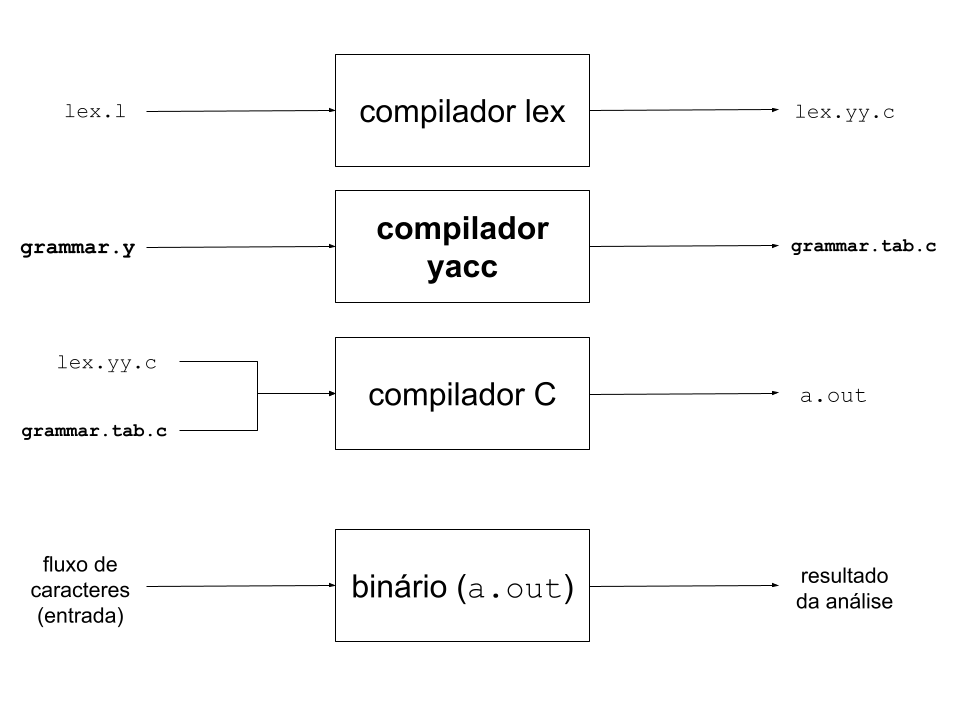
\includegraphics[scale=.35]{yacc-compilador.png}}

\begin{frame}[fragile]{Seções do arquivo}
\begin{lstlisting}
declarações

%%

regras gramaticais e ações

%%

código em C

\end{lstlisting}
\end{frame}

\subsection{Exemplo de especificação de gramática}

\frame{\tableofcontents[currentsubsection]}

\begin{frame}[fragile]{Exemplo}{Expecificação de gramática usando yacc}

  {\hfil\color{gray} Calculadora de mesa simples}\bigskip

  \begin{columns}
    \begin{column}{.35\textwidth}
      \begin{block}{Gramática}
        \begin{tabbing}
          E \= $\rightarrow$ \= E + T \= | T \\
          T \> $\rightarrow$ \> T * F \> | F\\
          F \> $\rightarrow$ \> ( E ) \> | {\bf digit}\\
        \end{tabbing}
      \end{block}
    \end{column}
    \scriptsize
    \pause
    \begin{column}{.65\textwidth}
      \begin{lstlisting}
%union {
        int d;
}
%token <d> DIGIT
%type  <d> expr term factor

%%
line   : expr '\n'         { printf("%d\n", $1); }
       ;
expr   : expr '+' term     { $$ = $1 + $3; }
       | term
       ;
term   : term '*' factor   { $$ = $1 * $3; }
       | factor
       ;
factor : '(' expr ')'      { $$ = $2; }
       | DIGIT
       ;
%%
      \end{lstlisting}
    \end{column}
  \end{columns}
\end{frame}

\note{O próximo slide é a explicação do bison executando em modo debug
  para a saída da calculadora de mesa simples.}
\begin{frame}{{\tt bison} LALR: exemplo}{reduções e deslocamentos}
\centering\small
  \begin{tikzpicture}[>=latex]
    \node (two) {{\tt 2}};
    \node (plus) [right of=two] {{\tt +}};
    \node (one) [right of=plus] {{\tt 1}};
    \node (times) [right of=one] {{\tt *}};
    \node (three) [right of=times] {{\tt 3}};
    \node (nl) [right of=three] {{\tt '$\backslash$n'}};
    \only<-5>{
      \node (pointer) [below of=two] {};
      \draw[->] (pointer) -- (two);
    }
    \only<6>{
      \node (pointer) [below of=plus] {};
      \draw[->] (pointer) -- (plus);
    }
    \only<7-9>{
      \node (pointer) [below of=one] {};
      \draw[->] (pointer) -- (one);
    }
    \only<10>{
      \node (pointer) [below of=times] {};
      \draw[->] (pointer) -- (times);
    }
    \only<11-12>{
      \node (pointer) [below of=three] {};
      \draw[->] (pointer) -- (three);
    }
    \only<13-15>{
      \node (pointer) [below of=nl] {};
      \draw[->] (pointer) -- (nl);
    }
    \only<13>{
      \node (pointer) [below of=one] {$3$};
    }
    \only<14->{
      \node (pointer) [below of=one] {$5$};
    }
  \end{tikzpicture}\bigskip

  \scriptsize
  \begin{tabular}[h]{r|l|c|l}
    \toprule
    & \hfil pilha & entrada &\hfil ação \\
    \midrule
    (1) &   &\hfill {\bf digit} + {\bf digit} * {\bf digit}\$& desloca \\
    \only<2->{
    (2) &  {\bf digit} &\hfill + {\bf digit} * {\bf digit}\$ & reduz: $F\rightarrow$ {\bf digit} \\
    }
    \only<3->{
    (3) & $F$ &\hfill + {\bf digit} * {\bf digit}\$ & reduz: $F\rightarrow T$ \\
    }
    \only<4->{
    (4) & $T$ &\hfill + {\bf digit} * {\bf digit}\$ & reduz: $T\rightarrow E$ \\
    }
    \only<5->{
    (5) & $E$ &\hfill + {\bf digit} * {\bf digit}\$ & desloca \\
    }
    \only<6->{
    (6) & $E+$ &\hfill {\bf digit} * {\bf digit}\$ & desloca \\
    }
    \only<7->{
    (7) & $E+$ {\bf digit} &\hfill  * {\bf digit}\$ & reduz: $F\rightarrow$ {\bf digit} \\
    }
    \note{aqui lookahead no * para decidir a próxima ação}
    \only<8->{
    (8) &  $E+F$ &\hfill  * {\bf digit}\$ & reduz: $T\rightarrow F$ \\
    }
    \only<9->{
    (9) &  $E+T$ &\hfill  * {\bf digit}\$ & desloca \\}
    \note{aqui lookahead no digit para decidir a próxima ação}
    \only<10->{
    (10) & $E+T*$ &\hfill {\bf digit}\$ & desloca \\
    }
    \only<11->{
    (11) & $E+T*${\bf digit} &\hfill \$ & reduz: $F\rightarrow$ {\bf digit} \\
    }
    \only<12->{
    (12) & $E+T*F$ &\hfill \$ & reduz: $T\rightarrow T*F$ \\
    }
    \note{aqui lookahead no newline para decidir a próxima ação}
    \only<13->{
    (13) & $E+T$ &\hfill \$ & reduz: $E\rightarrow E+T$ \\
    }
    \only<14->{
    (14) & $E$ &\hfill \$ & desloca {\tt '$\backslash$n'} \\
    }
    \only<15->{
    (15) & $E${\tt '$\backslash$n'} &\hfill \$ & reduz: $L\rightarrow E${\tt '$\backslash$n'} \\
    }
    \only<16>{
    (16) & $L$ &\hfill \$ & aceita \\
    }


    & & & \\
   \bottomrule
  \end{tabular}
\end{frame}

\begin{frame}[fragile]{{\tt flex} + {\tt bison}}{lex + yacc}
  {\hfil\color{gray} Calculadora de mesa simples}\bigskip

  \begin{columns}
    \begin{column}{.45\textwidth}\scriptsize
\begin{lstlisting}
%%
[0-9]     { yylval.d = atoi(yytext);
            return DIGIT;
          }
[*+()\n]  { return yytext[0]; }
[ \t]     { ; /* ignore */ }
.         {
            yyerror("erro");
          }
%%
\end{lstlisting}
\end{column}\scriptsize
\begin{column}{.53\textwidth}
\begin{lstlisting}
%union {
        int d;
}
%token <d> DIGIT
%type  <d> expr term factor

%%
line   : expr '\n'      {
                         printf("%d\n", $1);
                        }
       ;
expr   : expr '+' term   { $$ = $1 + $3; }
       | term
       ;
term   : term '*' factor { $$ = $1 * $3; }
       | factor
       ;
factor : '(' expr ')'    { $$ = $2; }
       | DIGIT
       ;
%%
      \end{lstlisting}
    \end{column}
  \end{columns}
\end{frame}

\subsection{Conflitos}

\frame{\tableofcontents[currentsubsection]}

\begin{frame}[fragile]{Conflitos}

  $$E \rightarrow\ E\ +\ E\ |\ E\ *\ E\ |\ (E)\ |\ \text{\bf digit} $$

  \small

\begin{lstlisting}

%%
calc    :   expr '\n'      { printf("%d\n", $1); }
        ;

// conflito por ambiguidade
expr    : expr '+' expr     { $$ = $1 + $3; }
        | expr '*' expr     { $$ = $1 * $3; }
        | '(' expr ')'      { $$ = $2; }
        | DIGIT             { $$ = $1; }
        ;
%%

\end{lstlisting}
\end{frame}

\begin{frame}{Conflitos}{exemplo}
\centering\small
  \begin{tikzpicture}[>=latex]
    \node (two) {{\tt 2}};
    \node (plus) [right of=two] {{\tt +}};
    \node (one) [right of=plus] {{\tt 1}};
    \node (times) [right of=one] {{\tt *}};
    \node (three) [right of=times] {{\tt 3}};
    \node (nl) [right of=three] {{\tt '$\backslash$n'}};
    \only<-3>{
      \node (pointer) [below of=two] {};
      \draw[->] (pointer) -- (two);
    }
    \only<3->{
      \node (pointer) [below of=two,xshift=.25cm] {\bf\large\color{red}?};
    }
  \end{tikzpicture}\bigskip

  \scriptsize
  \begin{tabular}[h]{r|l|l|c|l}
    \toprule
    & \hfil pilha &\hfil símbolo & entrada &\hfil ação \\
    \midrule
    (1) & 0 &  &\hfill {\bf digit} + {\bf digit} * {\bf digit}\$& desloca \\
    \only<2->{
    (2) & 0 1 &   {\bf digit} &\hfill + {\bf digit} * {\bf digit}\$ & reduz: $E\rightarrow$ {\bf digit} \\
    }
    \only<3->{
    (3) & 0 6 &   $E$ &\hfill + {\bf digit} * {\bf digit}\$ & {\large\color{red}conflito} \\
    }
    & & & &\\
   \bottomrule
  \end{tabular}
\end{frame}

\begin{frame}[fragile]{Resolução de conflitos}
  $$E \rightarrow\ E\ +\ E\ |\ E\ *\ E\ |\ (E)\ |\ \text{\bf digit} $$

  \small

\note{
  Uma gramática ambígua tende a ser menor e mais fácil de ler.
  Por isso, o {\tt yacc} fornece um mecanismo para usá-la.
  \cite{holub}. (pg 182)
}

\lstset{emph={left},emphstyle=\color{red}\bf}
\begin{lstlisting}
// solução usando %left
// '*' precede '+'
%left '+'
%left '*'

%%
line    :   expr '\n'      { printf("%d\n", $1); }
        ;

expr    : expr '+' expr     { $$ = $1 + $3; }
        | expr '*' expr     { $$ = $1 * $3; }
        | '(' expr ')'      { $$ = $2; }
        | DIGIT             { $$ = $1; }
        ;
%%
\end{lstlisting}
\end{frame}

\begin{frame}{Associatividade}

  \begin{itemize}
    \item Esquerda: {\tt \%left}\\
      Exemplo: 3 - 2 - 1
     \bigskip
    \item Direita:  {\tt \%right}\\
     Exemplo: 2  ** 3 ** 2 \hfil (potenciação)
     \bigskip
    \item Não-associativo: {\tt \%nonassoc}\\
      Exemplo: 0 || 1 || 0  \hfil (operador lógico OR)
  \end{itemize}
\end{frame}

\begin{frame}[fragile]{Lista}

  Lista de expressões

 \begin{lstlisting}
%%

prog        :   expr_list             { }

expr_list   :   expr_list expr '\n'   { printf("%d ", $2); }
            |   expr '\n' 
            ;

%%
\end{lstlisting}
\end{frame}
 

\subsection{Etapas finais de compilação}
\frame{\tableofcontents[currentsubsection]}

\begin{frame}{Etapas finais de compilação}

  \begin{itemize}
  \item Processamento da tabela de símbolos;
  \item Geração de código de máquina ({\it assembly}):
    \begin{itemize}
    \item Intel x64;
    \item ARM;
    \item RISC-V;
    \item $\ldots$
    \end{itemize}
  \item Geração de programa e C a ser compilado e executado
    (linguagens interpretadas);
  \item Geração de código intermediário ({\it bytecode});
  \item Tratamentos de erros.
  \end{itemize}
\end{frame}

\subsection{Alternativas ao bison}
\frame{\tableofcontents[currentsubsection]}

\begin{frame}{Outros ambientes de compilação}
  \framesubtitle{alguns exemplos}
  \begin{itemize}
  \item {\it Parsers} para outras linguagens:
    \begin{itemize}
    \item ANTLR (Java);
    \item PEG (Python);
    \item PEG.js (Javascript);
    \item pest (Rust).
    \end{itemize}
  \item Infraestrutura de compilação LLVM:
    \begin{itemize}
    \item Julia;
    \item Rust;
    \item Swift.
    \end{itemize}
  \item Máquina virtual Java (JVM):
    \begin{itemize}
    \item Clojure;
    \item Scala;
    \item Groovy.
    \end{itemize}
  \end{itemize}
\end{frame}

\subsection*{Referências}

\begin{frame}{Referências}

  \begin{itemize}
  \item Alfred V. Aho, Monica S. Lam, Ravi Sethi, Jeffrey D. Ullman.
    Compiladores: Princípios, Técnicas e Ferramentas. Editora
    Pearson, 2$^a$ edição, 2007.

  \item Douglas Thain. \href{http://compilerbook.org}{Introduction to
      Compilers and Language Design}. Free 2nd edition, 2020.
    Disponível em {\tt http://compilerbook.org}

  \item John Levine.
    \href{https://www.oreilly.com/library/view/flex-bison/9780596805418/}{flex
      \& bison}. Editora O'Reilly, 2009.

  \item Allen I.\ Hollub.
   \href{https://holub.com/compiler/}{Compiler Design in C}.
    Prentice-Hall, 1990.

  \item {\tt Bison} home page {\tt http://www.gnu.org/software/bison/}, Free
    Software Foundation.
  \end{itemize}
 \end{frame}


\section*{Referência}
\begin{itemize}
\item Alfred V. Aho, Monica S. Lam, Ravi Sethi, Jeffrey
  D. Ullman. Compiladores: Princípios, Técnicas e Ferramentas. Editora
  Pearson, 2$^a$ edição, 2007.
\end{itemize}

\end{document}
